\documentclass{scrartcl}
\usepackage[utf8]{inputenc}
\usepackage[english]{babel}
\usepackage{amsmath} % for align
\usepackage[left=2cm, right=2cm, bottom=3cm, top=2.5cm]{geometry}
\usepackage{graphicx}
\usepackage{placeins}
\usepackage[usenames,dvipsnames]{xcolor}
\usepackage[hidelinks]{hyperref}
\usepackage{caption}
\usepackage{multirow}

\title{Photoelectrons in the LHC chambers}
\author{Philipp Dijkstal}
\setlength\parindent{0pt}
\setlength\parskip{5pt}

\graphicspath{{src/}{./}{plots/}}
% My personal latex commands

\newcommand{\HGC}[2]{
	\begin{center}
	\includegraphics[height=#1\textheight]{#2}
	\end{center}
	}

\newcommand{\WGC}[2]{
	\begin{center}
	\includegraphics[width=#1\textwidth]{#2}
	\end{center}
	}

\newcommand{\introframe}[1]{
    \begin{frame}
        \centering
        \Huge #1
    \end{frame}
}

\newcommand{\introsection}[1]{
    \section{#1}
    \introframe{#1}
}

\newcommand{\derivative}[2]{
    \frac{\text{d}#1}{\text{d}#2}
}



\begin{document}

\maketitle
\tableofcontents

\section{Introduction}

This report describes how photoemission seeding is implemented in PyECLOUD for the electron cloud buildup simulations, especially for the LHC arcs.
It is laid out which quantities are necessary as an input to the simulations and how they have to be specified.
Some of them are derived from the theory of synchrotron radiation, others are material properties taken from published experiment data.
Several papers about measurements for materials used for the LHC beam screens are discussed, in order to arrive at the properties that represent the best knowledge available.
A simulation study that has been performed with these parameters is presented.

Furthermore, possible changes to PyECLOUD are outlined, some of which have already been implemented and could get merged into the main branch of the code.



\section{Photoelectrons in PyECLOUD}
    
\subsection{Input parameters}
\label{sec:input}


In PyECLOUD, photoelectrons are generated simultaneously with the beam charge.
Figure~\ref{fig:input} shows the related input parameters of the code, these are explained in more details in the following pages.
%It can be specified how many electrons per proton are generated and how they are distributed around the 2D chamber walls.

\begin{figure}[tbh]
    \centering
    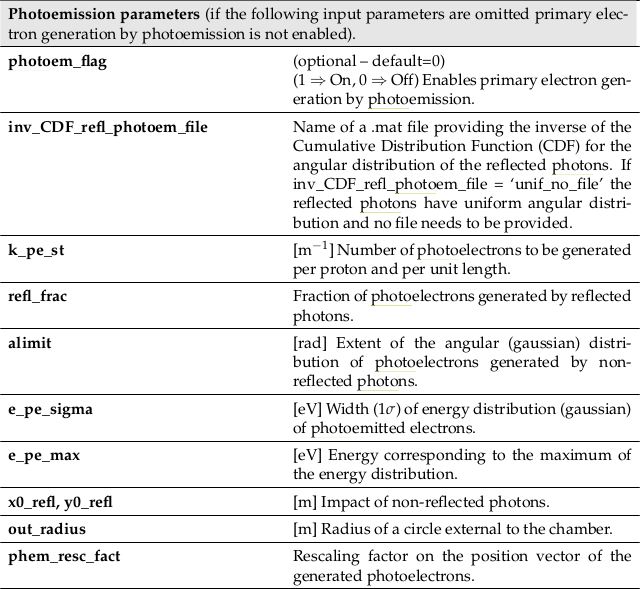
\includegraphics[width=0.8\textwidth]{../ss/pyecloud_doc.png}
    \caption{The input parameters of the PyECLOUD simulation code regarding photoemission seeding.}
    \label{fig:input}
\end{figure}

The quantity \textbf{k\_pe\_st} is the total number of photoelectrons per proton and m.
\\
The quantity \textbf{refl\_frac} is the ratio between all photoelectrons and those that origin from reflected photons.

The generation of photoelectrons created by immediately absorbed photons and reflected photons differs in PyECLOUD, see Fig.~\ref{fig:gt}.
For both of them, an angle relative to the center of the chamber is randomly generated.
In the case of non-reflected photons, this angle is Gaussian distributed with a standard deviation of \textbf{a\_limit}.
In the case of reflected photons, an angle of reflection with respect to the impact point is obtained from a given distribution.
The point where photoelectrons are generated is determined as the intersection of the line between a point on the outer circle  and the origin with a chamber wall.

\textbf{inv\_CDF\_refl\_photoem\_file} includes the inverse cumulative distribution function (CDF) for the angles under which the photons are reflected from the impact point.

Photoelectrons are emitted with a truncated Gaussian energy distribution, specified by \textbf{e\_pe\_sigma} and \textbf{e\_pe\_max} with only positive energies allowed.
Their initial direction is found through a cosine distribution for the angle with respect to the surface normal at these points.
\begin{figure}[tbh]
    \centering
    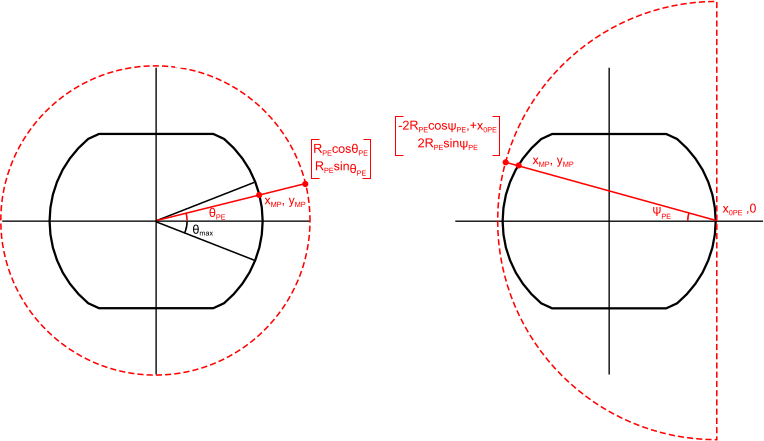
\includegraphics[width=0.8\textwidth]{../ss/gianni_thesis_photoelectrons.png}
    \caption{Position generation algorithm for photoelectrons from non-reflected (left) and reflected (right) photons~\cite{gianni}.}
    \label{fig:gt}
\end{figure}


\textbf{out\_radius} describes a circle that encloses the beam chamber, see Fig.~\ref{fig:gt}.

\textbf{x\_0\_refl} and \textbf{y\_0\_refl} are coordinates that have to be located inside the chamber.
This point together with an angle of reflectivity leads to the positions of new MPs from reflected photons, see Fig.~\ref{fig:gt}.
Cases where y\_0\_refl is nonzero are not supported, yet.

\subsection{Validation}

A script to generate the plots seen in Fig.~\ref{fig:test_module} is part of the "photoemission" branch of PyECLOUD on GitHub ("test\_photoemission.py").
It calls the photoemission module to produce these plots, and shows that the expected behavior is indeed achieved.
\begin{figure}[tbh]
    \centering
    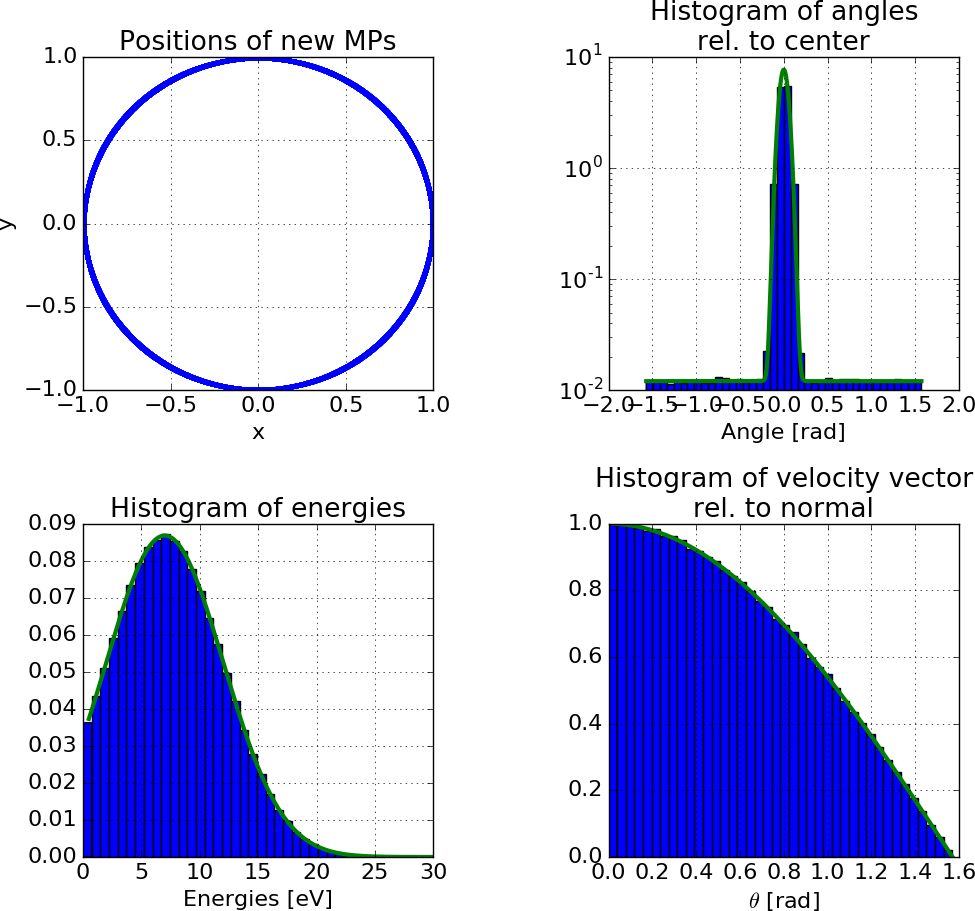
\includegraphics[width=0.8\textwidth]{../plots/test_module.png}
    \caption{
        The photoemission seeding is validated with these tests.
        The top two plots show the positions of new macroparticles for a circular chamber.
        The green line is the expected behavior for an alimit of 0.05 and a refl\_frac of 3.8\%, given a uniform distribution of reflected photons.
        The bottom plots show the energies and angles relative to the impact normal for new macroparticles.
    }
    \label{fig:test_module}
\end{figure}



\clearpage
\section{Photons emitted by the beam}
    
To estimate the number of photoelectrons in the LHC beam pipe, the amount of photons generated by the beam has to be calculated first.
The equations necessary for this were found in~\cite{hofmann}.

Eq.~(5.40) in this reference describes the power spectrum of the radiation emitted by the beam.
\begin{align}
    \derivative{P}{\omega} = \frac{P_s}{\omega_c} S_s(\frac{\omega}{\omega_c})
    \label{eq:dp}
\end{align}
$P_s$ and $\omega_c$ are the total power emitted in the bend and the critical frequency of the radiation:
\begin{align}
    P_s &= \frac{e^2}{4\pi\epsilon_0}\frac{2c\gamma^4}{3\rho^2}
    \label{eq:ps}
    \\
    \omega_c &= \frac{E_c}{\hbar} = \frac{3c\gamma^3}{2\rho}
    \label{eq:omega_c}
    \\
    \frac{P_s}{\omega_c} &= \frac{e^2\gamma}{9\pi\epsilon_0\rho}
\end{align}
An approximation here is $\beta\approx1$, certainly fulfilled for any accelerator that emits significant synchrotron radiation.
The function $S_s$ is an integral over a modified Bessel function.
\begin{align}
    S_s(x) = \frac{9\sqrt{3}}{8\pi} x \int_x^\infty \text{d}z'\ K_{5/3}(z')
    \label{eq:s_s}
\end{align}
The spectrum is easily transformed from frequency to number of photons with the relation $P(\omega)=\dot{n}\hbar\omega$.
Integration yields the number of photons above a certain energy, for example the work function of a material.
\begin{align}
    \derivative{\dot{n}}{\omega} &= \frac{P_s}{\omega_c} \frac{1}{\hbar\omega}S_s(\frac{\omega}{\omega_c})
    \label{eq:nomega}
    \\
    \dot{n} &= \frac{P_s}{E_c}\int_{\omega_\text{min}}^\infty \text{d}\omega \frac{1}{\omega} S_s(\frac{\omega}{\omega_c})
    \\
    &= \frac{P_s}{E_c}\int_{\omega_\text{min}/\omega_c}^\infty \text{d}x \frac{1}{x} S_s(x)
    \\
    &= \underbrace{\frac{P_s}{E_c}  \frac{9\sqrt{3}}{8\pi}}_{=\frac{\sqrt{3}}{8\pi^2\hbar}\frac{e^2\gamma}{\epsilon_0\rho}}
    \cdot
    \underbrace{\int_{\omega_\text{min}/\omega_c}^\infty \text{d}x  \int_x^\infty \text{d}z' K_{5/3}(z')}_{=A(\omega_\text{min}/\omega_c) = A(x_\text{min})}
\end{align}
The double integral $A(\omega_\text{min}/\omega_c)$ can be transformed to a single integral.
\begin{align}
    A(x_\text{min}) &= \int_{x_\text{min}}^\infty \text{d}x  \underbrace{\int_x^\infty \text{d}z'\ K_{5/3}(z')}_{=F(x)}
    \\
    &=\int_{x_\text{min}}^\infty \text{d}x\ F(x) \cdot 1
    \\
    &= \underbrace{\lim_{b\rightarrow \infty}F(b) \cdot b}_{=0} - F(x_\text{min}) \cdot x_\text{min} - \int_{x_\text{min}}^\infty \text{d}x\ F'(x) \cdot x
    \\
    &= - \int_{x_\text{min}}^\infty \text{d}x\ K_{5/3}(x) \cdot x_\text{min} - \int_{x_\text{min}}^\infty \text{d}x\ (-K_{5/3}(x)) \cdot x
    \\
    &= \int_{x_\text{min}}^\infty \text{d}x\ K_{5/3}(x) (x-x_\text{min})
\end{align}
The number of photons per m in a dipole with constant field is obtained by applying a factor of $1/c$ to $\dot{n}$.
\begin{align}
    n_\gamma = \derivative{n}{z} = \frac{\sqrt{3}}{8\pi^2}\frac{e^2\gamma}{\hbar c \epsilon_0 \rho}
    \cdot
    \int_{\omega_\text{min}/\omega_c}^\infty \text{d}x\ K_{5/3}(x) (x-\frac{\omega_\text{min}}{\omega_c})
    \label{eq:ngamma}
\end{align}
Another interesting feature is the angular distribution of photons.
Far above the critical angle, emission of synchrotron radiation is negligible.
\begin{align}
    \theta_c(\omega)
    = \frac{1}{\gamma}\left( \frac{2\omega_c}{\omega} \right)^{1/3}
    = \left( \frac{3c}{\rho\omega} \right)^{1/3}
    \label{eq:crit_angle}
\end{align}
For energies corresponding to the copper work function, the critical angle is about 0.36~mrad.

Figure~\ref{fig:n_photons} shows the properties of some functions that were presented previously.
It is created with a script in the python module that is related to this report \cite{cellinput}.
\begin{figure}[tbh]
    \centering
    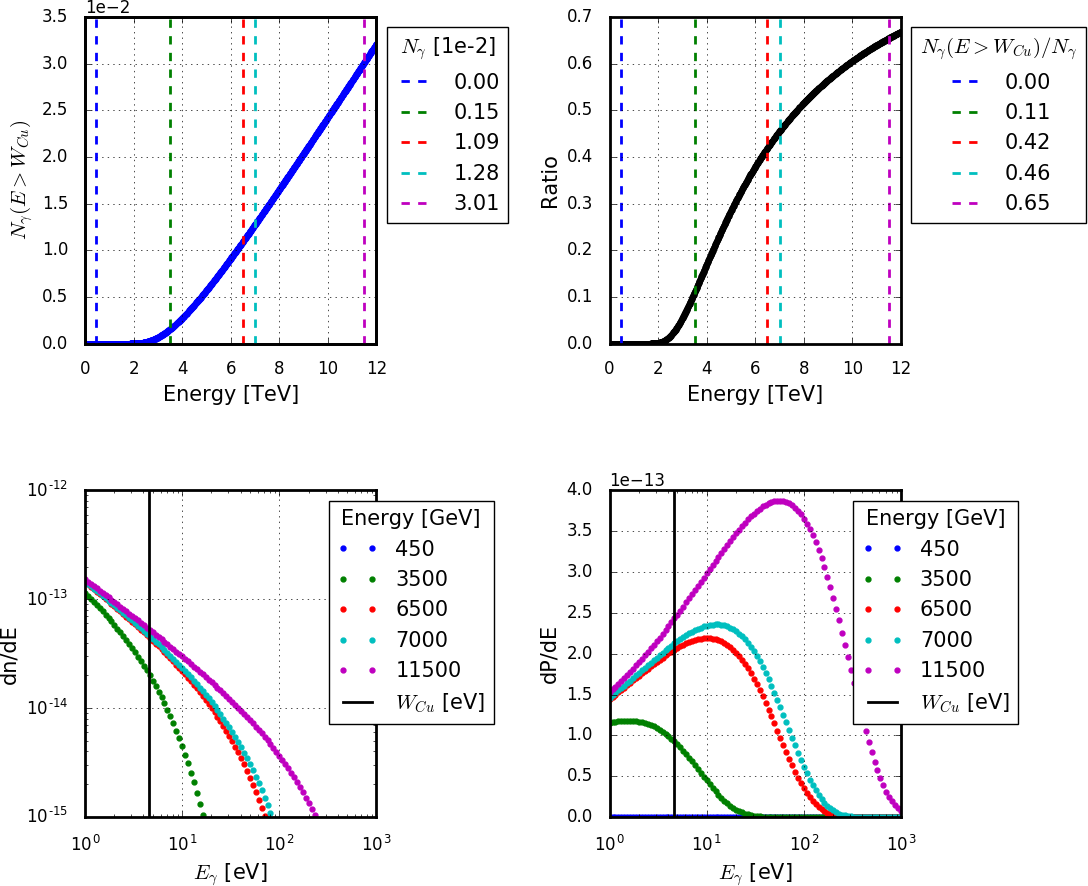
\includegraphics[width=\textwidth]{./plots/n_photons.png}
    \caption{
        Top left: Number of photons above the copper work function in the LHC.
        Top right: Ratio of photons above the copper work function.
        Bottom left: Distribution of photons for various beam energies.
        Bottom right: Energy distribution of impinging photons.
    }
    \label{fig:n_photons}
\end{figure}



\clearpage
\section{Distributions of photons in the LHC chamber}
	
\subsection{LHC chamber with sawtooth structure}
The transverse geometry of the LHC chamber is pictured in Fig.~\ref{fig:beam_screen_structure}.
Of great importance is the sawtooth structure that ensures an almost normal impact of most photons on the surface, greatly reducing the reflectivity.
Therefore, most photoelectrons are created at the outer part of the beam screens, where they do not significantly contribute to the electron cloud buildup.


\begin{figure}[tbh]
    \centering
    \begin{minipage}[c]{0.47\textwidth}
        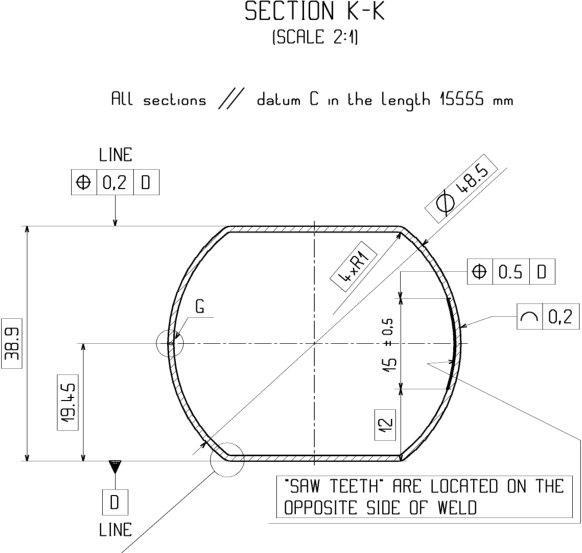
\includegraphics[width=\textwidth]{../ss/beam_screen_drawing.png}
    \end{minipage}
    \hspace{0.5cm}
    \begin{minipage}[c]{0.47\textwidth}
        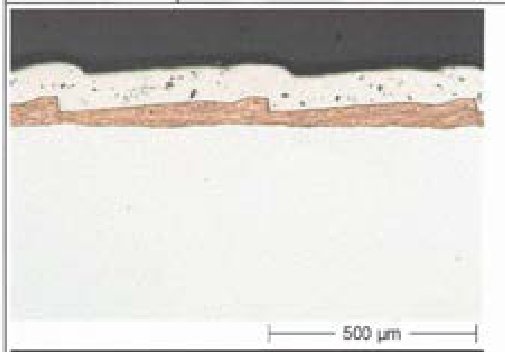
\includegraphics[width=\textwidth]{../ss/sawtooth_fine.png}
    \end{minipage}
\caption{
		Left: the technical drawing of the LHC beam screen~\cite{beam_screen_drawing}. Right: a closeup of the sawtooth structure. The vertical edges are about 35~$\mu$m long~\cite{zimmermann}.
		}
\label{fig:beam_screen_structure}
\end{figure}


\subsection{SynRad3D simulations}
The azimuthal distributions of absorbed photons in the LHC chamber have been simulated with the code SynRad3D~\cite{guillermo}.
The photons origin from a beam with 7~TeV energy, and only photons with more than 4~eV energy are considered.
The results are shown in Fig.~\ref{fig:guillermo}.
With access to the raw data, it could be converted to the PyECLOUD input parameter \textbf{inv\_CDF\_refl\_photoem\_file}.

\begin{figure}[tbh]
    \centering
    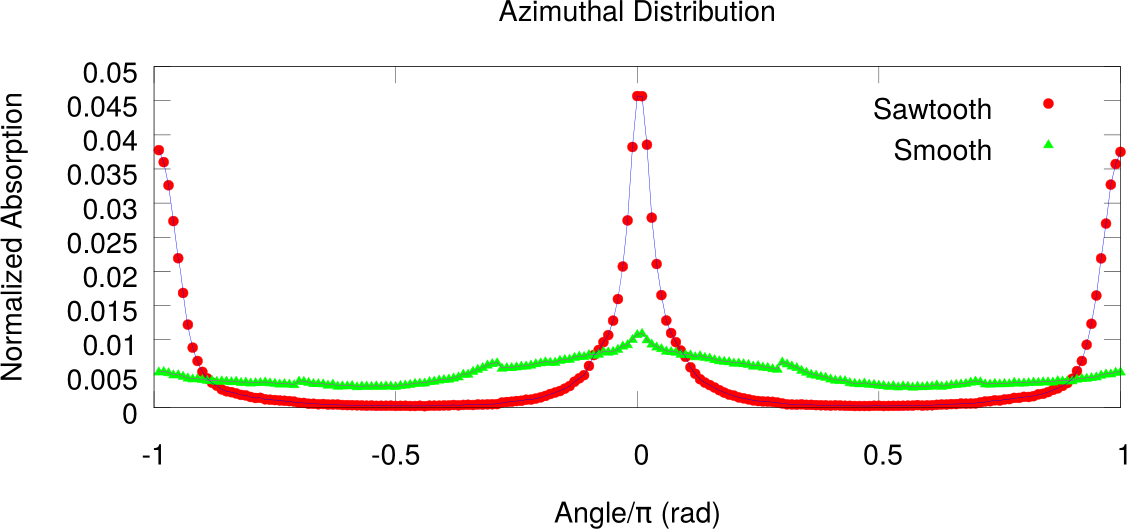
\includegraphics[width=0.8\textwidth]{../ss/photon_distribution_guillermo.png}
	\caption{The photon distribution as it was simulated for the LHC chamber geometry with and without sawtooth~\cite{guillermo}.
	An angle of 0 corresponds to the impact point of the synchrotron radiation.}
    \label{fig:guillermo}
\end{figure}


\subsection{Other simulations}



\clearpage
\section{Emission of photoelectrons from the LHC beam screen material}
	
Several papers on relevant material properties are discussed in this section.
The following notation is used in most of them
\begin{align}
    R &= \frac{n_{\gamma, \text{reflected}}}{n_{\gamma, \text{incident}}}
    \label{eq:not1}
    \\
    Y &= \frac{N_e}{n_{\gamma, \text{incident}}}
    \\
    Y^* &= \frac{N_e}{n_{\gamma, \text{absorbed}}} = \frac{Y}{1-R}
    \label{eq:yy}
\end{align}


    \subsection{Baglin, Collins, Gröbner 1998 (CERN)}
\label{sec:Baglin}

The properties of several materials, including co-laminated copper with and without sawtooth structure, were studied regarding photon reflectivity and photoelectron yield per photon~\cite{baglin}.

\subsubsection{Experiment setup}

\begin{figure}[tbh]
    \centering
    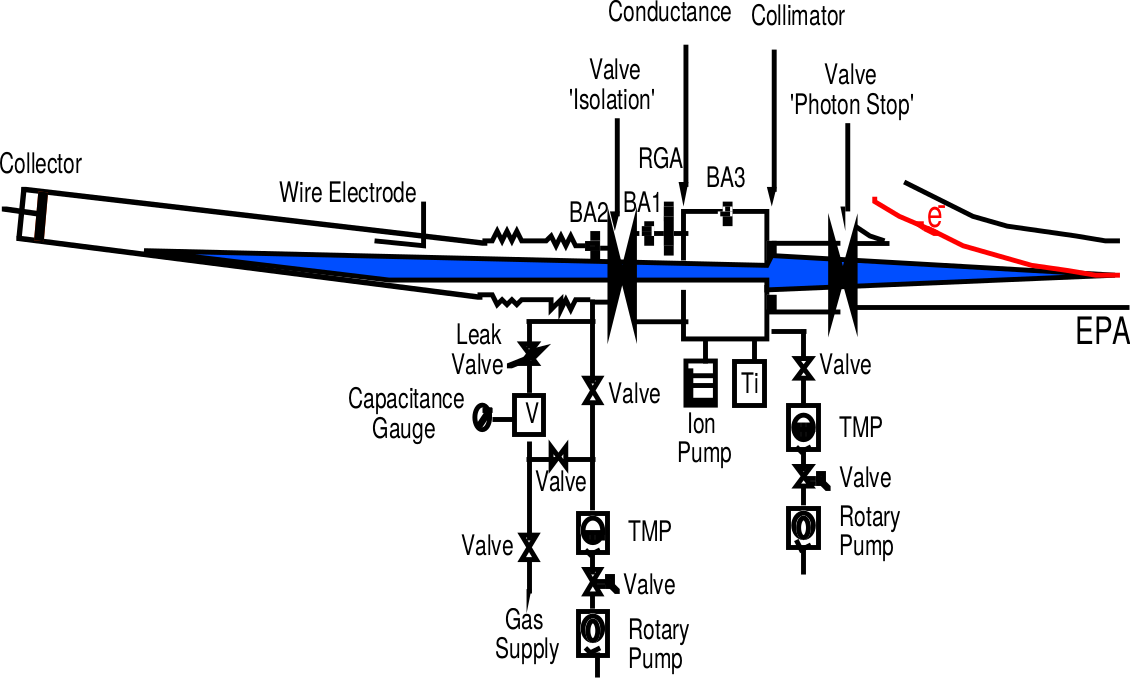
\includegraphics[width=0.8\textwidth]{../ss/experiment_baglin.png}
    \caption{Experiment setup of the paper presented in Sec.~\ref{sec:Baglin}.}
    \label{fig:exp}
\end{figure}


Fig.~\ref{fig:exp} shows the experiment setup.
It was possible to measure forward reflectivities and photoelectron yields.
The collimator is of square geometry and 11~mm wide.
The authors write:
\begin{quote}
    \small
    Due to the vertical collimation, photon energies below about 4 eV are attenuated.
\end{quote}

The photoelectrons are measured at the collector, either after direct impact or after a reflection as shown in the figure.
The ratio of the two currents is the photon reflectivity, where the backwards reflected photons are neglected (see Sec.~\ref{sec:Mahne}).

The report cites that for radiation with a critical energy of 45 and 194~eV, corresponding to 7 and 11.5~TeV LHC beams, the number of photons is multiplied by 0.46 and 0.65, respectively.
This exactly coincides with the ratio of photons above the work function with respect to all photons, see Fig.~\ref{fig:n_photons}.



\subsubsection{Results}
The results of this paper are given in Fig.~\ref{fig:baglin_table}.
Note that the photoelectrons per incident photon $Y$ has been measured, which was then transformed to the photoelectrons per absorbed photon, $Y^*$.
The reflectivity $R$ was measured at an incidence angle of 11~mrad for the sample without sawtooth.


\begin{figure}[tbh]
    \centering
    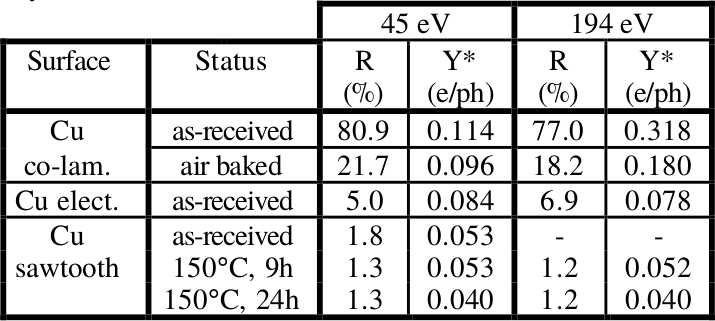
\includegraphics[width=0.4\textwidth]{../ss/baglin_table.png}
    \caption{
        The main results of the paper from Sec.~\ref{sec:Baglin}, surface properties for different materials when radiated by two different photon distributions, characterized by the critical photon energy. 
        R is the fraction of reflected photons, Y$^*$ the electron yield per absorbed photon.}
    \label{fig:baglin_table}
\end{figure}

\subsubsection{Open questions}
\begin{enumerate}
    \item
        The authors claim that the photons were sent through a collimator with 11x11~mm size, leading to the photons below 4~eV to be attenuated.
        %The resulting minimum photon energy from a maximum of 11~mm wavelengths can be calculated.
        %\begin{align}
        %    E = \frac{ch}{\lambda} = 1.2\cdot10^{-4}~\text{eV}
        %\end{align}
        %In order to attenuate photon energies below 4 eV, the collimation would have to be about 0.2~$\mu$m.
        It is not clear how exactly the low energy photons were attenuated, or why this would have been necessary.
    \item
        The photon induced scrubbing of the surface was not subject of this paper.
        The photon flux or integrated photon dose is not stated.
        The photoelectron yields that are quantified in this paper should probably be used as an upper limit.
    \item
        Considering the paper from Sec.~\ref{sec:Mahne}, the real reflectivity of the samples, especially with sawtooth, is expected to be higher.
        Because $Y^*$ and $R$ are not independent, $Y^*$ should maybe be updated (increased) according to Eq.~(\ref{eq:yy}).
\end{enumerate}


    \subsection{Baglin, Collins, Gröbner, Grünhagel et al. 2001 (CERN)}
\label{sec:Baglin2}
Photon-induced scrubbing is quantified with the same measurement apparatus as presented in Sec.~\ref{sec:Baglin}~\cite{baglin2}.
Again, co-laminated copper with and without sawtooth was subject of these studies, however only the results for the material with included sawtooth are fully reported.

\subsubsection{Experiment setup}
Copper samples were irradiated with light from the Electron-Positron Accumulator (EPA, now dismantled) and their reflectivities and photoelectron yields were measured in the same way as in Sec.~\ref{sec:Baglin}.
The sample consisted of a Cu sawtooth structure.


\subsubsection{Results}

Figure~\ref{fig:baglin2_scrubbing} shows the results from the measurements of this paper.
There are clear differences in the reflectivity, which is much higher than in Fig.~\ref{fig:baglin_table}.
This implies that the yield is much smaller and the reflectivity much higher than before.
Furthermore they document the photon scrubbing after a dose of 1.5~$\cdot10^{22}$ photons, corresponding to about 600~h of LHC operations, as stated in the paper.
After this, the yield is about halved.
However the full results indicate that this process has not even saturated and could possibly be going even further, see Fig.~\ref{fig:baglin2_scrubbing}.
There seems to be no effect on the reflectivity.

\begin{figure}[tbh]
    \centering
    \begin{minipage}[c]{0.37\textwidth}
        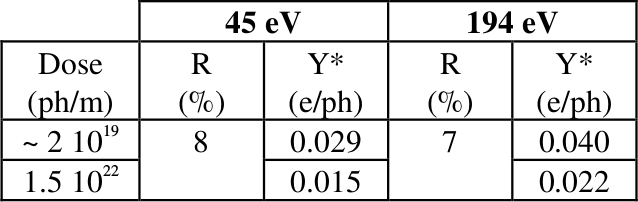
\includegraphics[width=\textwidth]{../ss/experiment_baglin2.png}
    \end{minipage}
    \hspace{0.5cm}
    \begin{minipage}[c]{0.57\textwidth}
        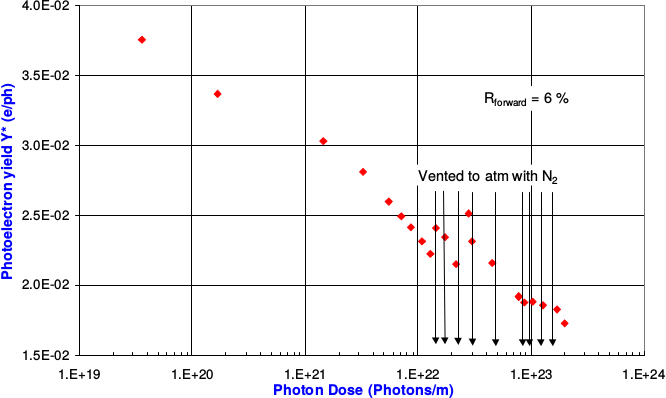
\includegraphics[width=1\textwidth]{../ss/photoelectron_scrubbing_baglin2.png}
    \end{minipage}
    \caption{
        Left: the reflectivities and photoelectron yields from the measurements of Copper samples with sawtooth presented in Sec.~\ref{sec:Baglin2}.
        \\
        Right: the impact of photon scrubbing on the photoelectron yield.
    }
    \label{fig:baglin2_scrubbing}
\end{figure}


The differences to the paper discussed in Sec.~\ref{sec:Baglin}, performed with the same experiment setup, is explained with the conditioning by reflected photons during the previous experiments.

\subsubsection{Open questions}

\begin{enumerate}
    \item It is stated that Cu co-lam. without sawtooth has been subject to this study as well, yet these results are not published.
\end{enumerate}


    
\subsection{Mahne, Baglin, Collins et al. 2004 (ELETTRA)}
\label{sec:Mahne}
This paper~\cite{mahne} covers only the photon reflectivity distributions, these were measured at ELETTRA, Italy.

\subsubsection{Experiment setup}
The experiment discussed in this paper is based on measured photons instead of electrons, see Fig.~\ref{fig:exp_mahne}.
Copper samples with and without sawtooth were irradiated with synchrotron light between 8 and 200~eV.
The reflectivity of the samples were measured in different directions.
The electron yields however could not be recorded.

\begin{figure}[tbh]
    \centering
    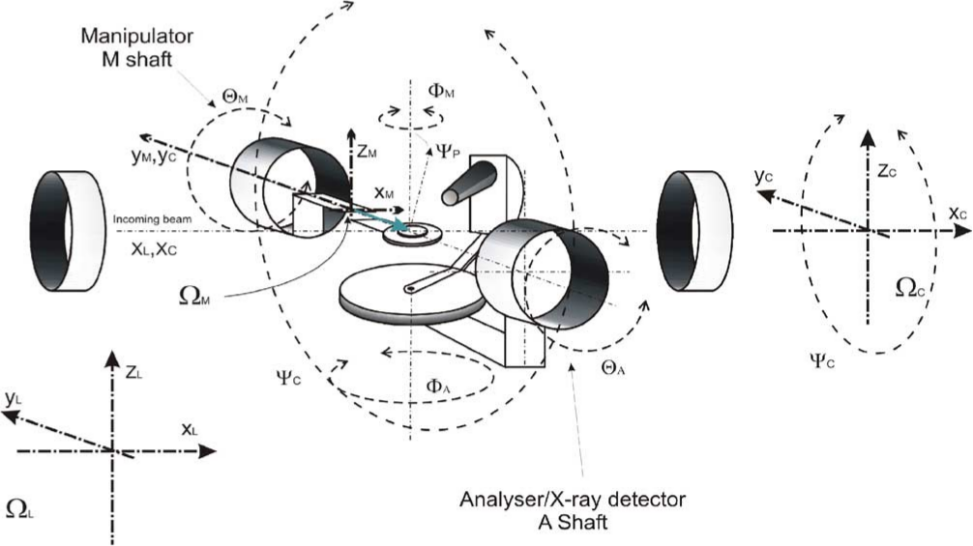
\includegraphics[width=0.8\textwidth]{../ss/experiment_mahne.png}
    \caption{The experiment setup from Sec.~\ref{sec:Mahne}.}
    \label{fig:exp_mahne}
\end{figure}


\subsubsection{Results}

The main results are listed in Fig.~\ref{fig:mahne}.
First, the reflectivity depending on the angle is shown for synchrotron radiation with a critical energy of 44~eV, similar to the previously discussed paper from Baglin et al.
The difference is that not only the reflectivity in forward direction was measured, but in all directions.
Figure~\ref{fig:mahne} (bottom) specifies the total reflectivity.
In case of the sawtooth, reflectivity increases from 1.8\% to 10\%.

Furthermore, it was found that the reflectivity depends on the photon energy.
This means that also the spectrum of reflected photons is different from the original one.


\subsubsection{Open questions}
Some inconsistencies exist.
\begin{itemize}
    \item The Baglin paper from Sec.~\ref{sec:Baglin} measured reflectivity as 1.8\% for the sawtooth sample, whereas the forward scattering in this paper alone amounts to 4\%.
    \item Furthermore, it is unclear how the 2\% diffused photons are obtained from a white light spectrum.
        In Fig.~\ref{fig:mahne} (right), the amount of diffused photons never reaches 2\% for any photon energy.
        %Certainly, the 2\% cannot be reached for a spectrum of photons, either.
        This discrepancy is not commented in the paper.
    \item The photon flux is not stated, photon scrubbing is not mentioned.
\end{itemize}


\begin{figure}[tbh]
    \centering
    \begin{minipage}[c]{0.47\textwidth}
        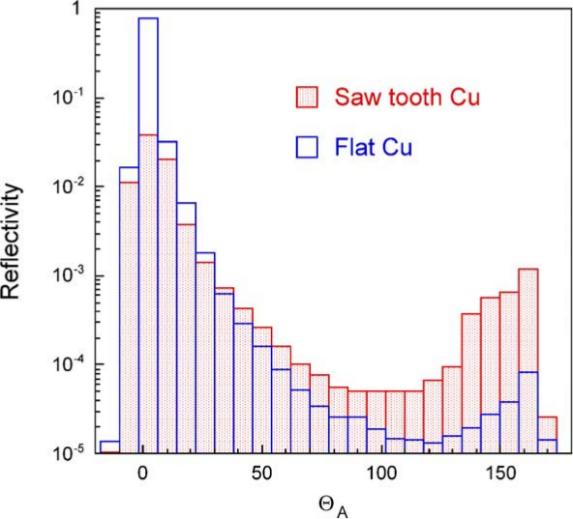
\includegraphics[width=\textwidth]{../ss/mahne_refl.png}
    \end{minipage}
    \hspace{0.5cm}
    \begin{minipage}[c]{0.47\textwidth}
        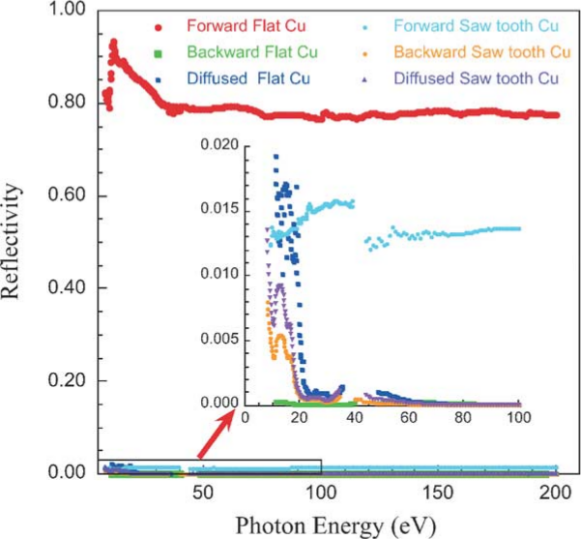
\includegraphics[width=\textwidth]{../ss/mahne_yield.png}
    \end{minipage}

    \begin{minipage}[c]{0.48\textwidth}
        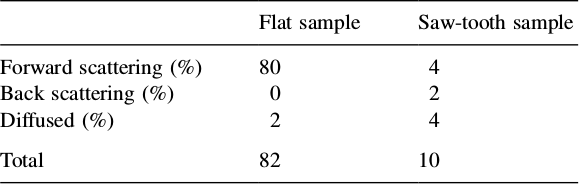
\includegraphics[width=\textwidth]{../ss/mahne_table.png}
    \end{minipage}
    \caption{
        Left: Measured reflectivity of Cu samples for different angles after grazing incidence.
        \\
        Right: Measured electron yield of Cu samples.
        \\
        Bottom: Summary of reflectivities for a LHC-type spectrum from the paper presented in Sec.~\ref{sec:Mahne}.
    }
    \label{fig:mahne}

\end{figure}




    
\subsection{Cimino, Collins, Baglin 1999 (BESSY)}
\label{sec:Cimino}

This very long paper~\cite{cimino} covers many interesting aspects.
\begin{itemize}
    \item kinetic energy of photoelectrons
    \item angular spectrum of photoemission
    \item dependence of emission on photon energy
    \item photoemission yields
    \item impact of photon scrubbing on yields and kinetic energies
\end{itemize}
Many materials were studied, among those is Copper but without sawtooth structure.

\subsubsection{Experiment setup}

Potentially monochromatic synchrotron radiation is guided to the experimental station.
The reflectivity is not measured or taken into account.
This means that the yields correspond to photoelectrons per incident photons $Y$.

\begin{figure}[tbh]
    \centering
    \begin{minipage}[c]{0.65\textwidth}
    	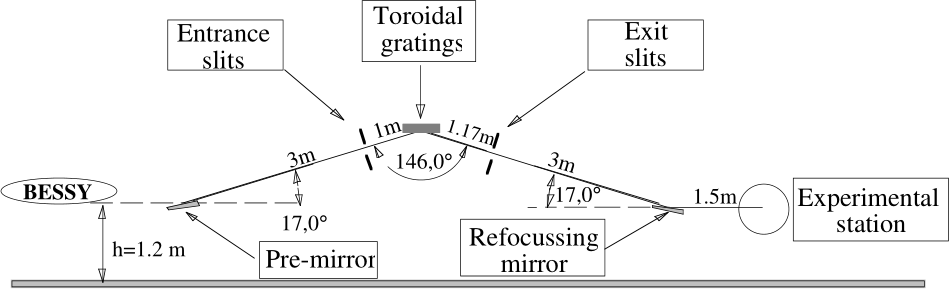
\includegraphics[width=1\textwidth]{../ss/cimino_setup.png}
    \end{minipage}
    \hspace{0.5cm}
    \begin{minipage}[c]{0.30\textwidth}
    	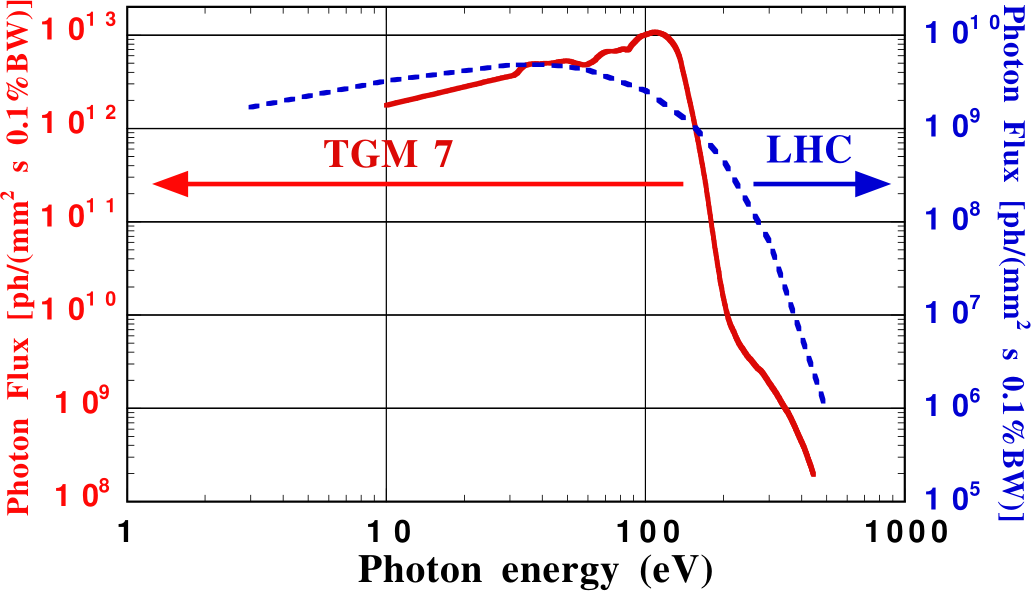
\includegraphics[width=1.0\textwidth]{../ss/cimino_wl_spectrum.png}
    \end{minipage}
    \caption{Left: The experiment setup for the paper presented in Sec.~\ref{sec:Cimino}. Right: The white light spectrum of the SR source.}
    \label{fig:cimino_setup}
\end{figure}


\subsubsection{Results}

The kinetic energy spectra of photoelectrons from Copper were measured before and after scrubbing with white light, see Fig.~\ref{fig:cimino_cu_spectrum}.
It is notable that the photoelectron yields $Y$ are much higher than those presented in Sec.~\ref{sec:Baglin}.
%This can be seen in Tab.~\ref{tab:input_table}, where $Y$ was recovered from the measurement of Sec.~\ref{sec:Baglin} as 2.3$\cdot10^{-2}$, whereas it is around 10 to 6$\cdot10^{-2}$ for as-received and scrubbed samples in this paper.
Regarding the spectra of kinetic energy, it becomes clear that white light scrubbing has a similar effect as surface cleaning with Argon sputtering.
Especially the output of low energy photoelectrons is diminished, meaning that also the total yield decreases significantly.

\begin{figure}[tbh]
    \centering
\end{figure}
\begin{figure}[tbh]
    \centering
    \begin{minipage}[c]{0.47\textwidth}
    	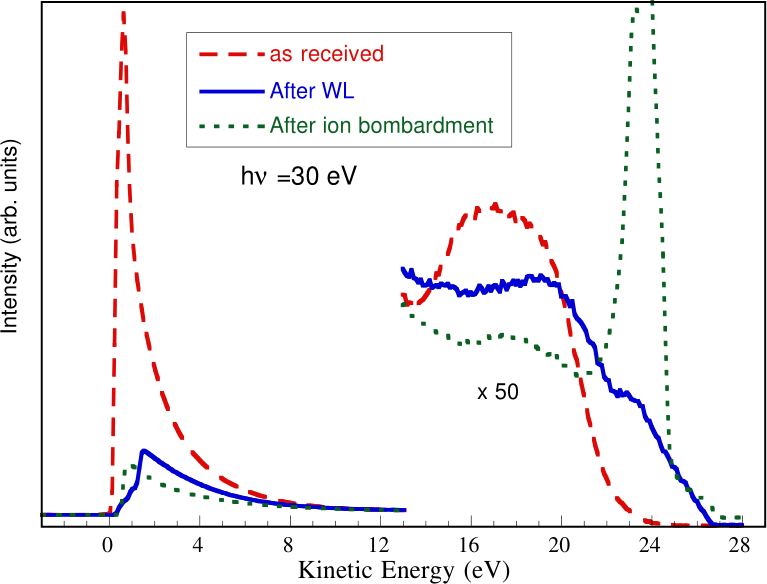
\includegraphics[width=1.0\textwidth]{../ss/cimino_cu_spectrump.png}
    \end{minipage}
    \hspace{0.5cm}
    \begin{minipage}[c]{0.47\textwidth}
        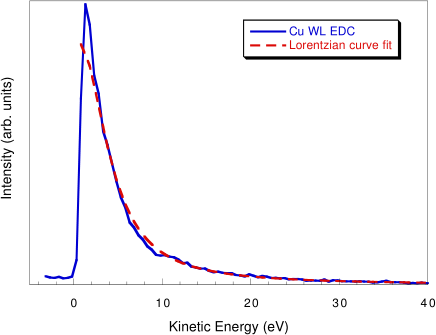
\includegraphics[width=\textwidth]{../ss/cimino_cu_fit.png}
    \end{minipage}
    \begin{minipage}[c]{0.7\textwidth}
        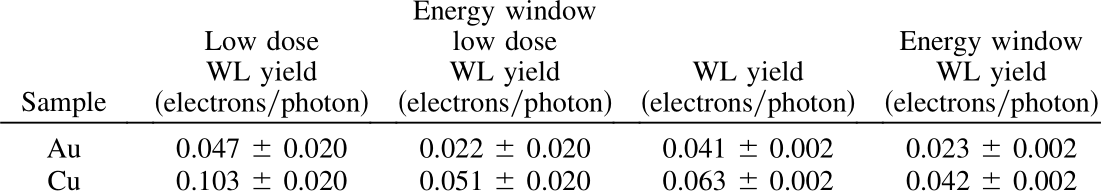
\includegraphics[width=\textwidth]{../ss/cimino_table.png}
    \end{minipage}
    \caption{
        Left: The photoemission spectra for 30~eV photons on Copper (Sec.~\ref{sec:Cimino}).
        The blue curve corresponds to a state after scrubbing has been performed, it is similar to the spectrum after a surface cleaning with ion bombardment.
        \\
        Right: A Lorentzian fit to the low-dose WL spectrum centered at 0.64~eV and 3.7~eV wide.
        \\
        Bottom: WL photoelectron yields for Au and Cu.
        The energy window corresponds to photoelectrons with energies between 1 and 6~eV.
        After WL scrubbing, the yield decreases by about 40\%.
		}
    \label{fig:cimino_cu_spectrum}
\end{figure}




\clearpage
\section{Proposed changes for PyECLOUD}
    
\subsection{Cosine Theta distribution}
\label{sec:cosine3D}
As mentioned in Sec.~\ref{sec:input}, the emission angle of photoelectrons in PyECLOUD is meant to follow a cosine distribution:
\begin{align}
    \derivative{n}{\Omega} &\propto \cos\theta
    \\
    \text{d}\Omega_{2D} &= \text{d}\theta
    \\
    \text{d}\Omega_{3D} &= \sin\theta~\text{d}\theta~\text{d}\varphi
    \label{eq:angles}
\end{align}
In PyECLOUD, the two-dimensional case is implemented even though the buildup process really happens in 3D space.
On average, this leads to too small angles (see Fig.~\ref{fig:distribution}), and is a common error in 2D simulation codes~\cite{angle}.
It impacts the buildup simulations because it influences the time necessary for a photoelectron to reach the opposing wall of the chamber, and potentially be absorbed there.
A branch on GitHub named "angle\_cosine3" changes this behavior.
%TODO
%
%

\begin{figure}[tbh]
    \centering
    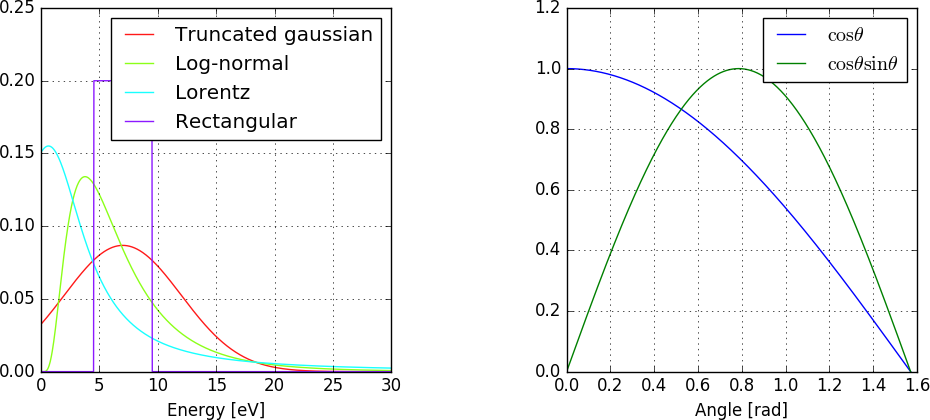
\includegraphics[width=0.8\textwidth]{../plots/distributions.png}
    \caption{
        The left plot shows a cut-off normal distribution characterized by a width and a standard deviation.
        A log-normal distribution with the same mean and variance as the undistorted Gaussian distribution is shown in green.
    The log-normal distribution does not extend to negative values.
    }
    \label{fig:distribution}
\end{figure}


\subsection{Delayed photoelectron production}
\label{sec:delay}

In PyECLOUD, photoelectrons are generated in parallel to the beam charge.
This means that the difference in path length is not considered.
Until a photon hits the chamber wall, the bunch has moved further due to the bending, see Fig.~\ref{fig:drawing}.
\begin{figure}[tbh]
    \centering
    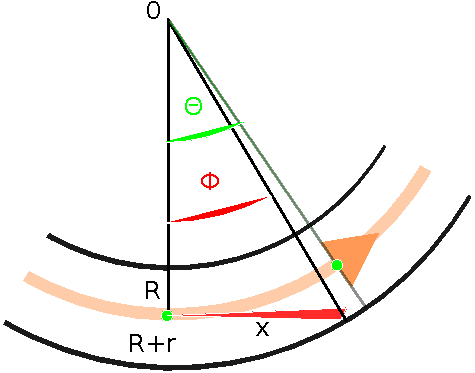
\includegraphics[width=0.5\textwidth]{../scripts/drawing.pdf}
    \caption{The path difference between protons (green) and photons(red).}
    \label{fig:drawing}
\end{figure}
The path difference is calculated in the following way, where $R=2803.95$~m for the LHC, and $r=22$~mm.
$x$ is the distance travelled by the photons before the wall is reached.
\begin{align}
    (R+r)^2 &= R^2 + x^2
    \\
    x &= \sqrt{2Rr + r^2} = 11.1~\text{m}
    \\
    \Phi &= \tan\frac{x}{R} = 0.00396136
    \\
    \Theta &= \frac{x}{R} = 0.00396134
    \\
    \Delta t &= \frac{R(\Theta - \Psi)}{c} = 1.938\cdot10^{-13}~s
\end{align}
This path difference is negligible as it is much smaller than a time step in the simulation, normally around $10^{-11}$~s.

Furthermore, photons that are absorbed only after (multiple) reflections (note that the reflection coefficient for grazing incident photons on Copper without sawtooth is larger than 80\%) are delayed with respect to the originating beam charge.
One reflection in normal direction causes to a delay of $\Delta t = \frac{2r}{c} = 1.48\cdot10^{-10}$~s, insignificant with respect to the bunch spacing of $2.5\cdot10^{-8}$, but longer than a time step in the simulations.
Backward or forward reflections, as indicated in Fig.~\ref{fig:synrad} could however lead to 
% TODO
% continuous photoemission


\subsection{Energy of new photoelectrons}

The energy of newly created photoelectrons is not very relevant in the current implementation of PyECLOUD, as they are immediately accelerated to much higher energies by the electric field of the beam charge.
If however a delayed photoemission was implemented, it could become more important.

The currently used truncated Gaussian for the energy distribution is not supported by laboratory measurements.
Other distributions have been introduced to the branch "photoemission", available on GitHub.
These are specified by the new input parameter \textbf{energy\_distribution}, which allows to choose from the following options in addition to the truncated Gaussian:
\begin{itemize}
    \item a log-normal distribution, which is also used for new secondary electrons.
        One advantage is that it does not have to be truncated, as negative energies cannot occur.
    \item a truncated Lorentzian, as indicated by Fig.~\ref{fig:cimino_cu_spectrum}.
        However it only fits well for the low-dose sample, otherwise the low-energy part is greatly reduced.
    \item a rectangular or a mono-energetic distribution in order to study the impact.
\end{itemize}
Figure~\ref{fig:distribution} visualizes the first three approaches, while Fig.~\ref{fig:test_energy_dist} shows a comparison of the resulting heat loads for different energy distributions, as well as the electron density
It shows that the initial energy of the photoelectrons hardly has an impact, at least with the current version of the code where photoelectrons are not created in between bunches.
Notable is the spike caused by the fat tail of the Lorentzian distribution, which is expected to generate photoelectrons with a very high energy from time to time, and should therefore be avoided.

\begin{figure}[tbh]
    \centering
    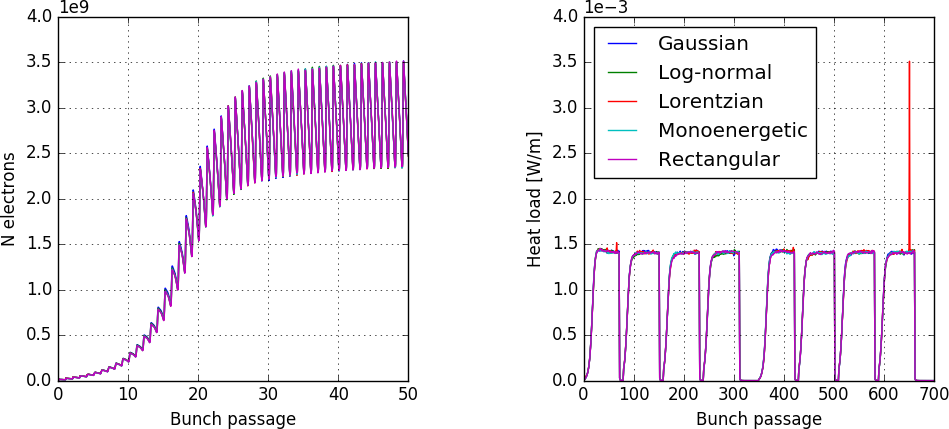
\includegraphics[width=0.8\textwidth]{../plots/energy_distribution_impact.png}
    \caption{
        The impact of several different energy distributions is compared for an e-cloud buildup simulation of the LHC chamber in a dipolar field at 6.5~TeV beam energy and nominal beam parameters.
        Left: The number of electrons in an electron-cloud buildup simulation.
        Right: The heat load per bunch passage.
    }
    \label{fig:test_energy_dist}
\end{figure}

Figure~\ref{fig:time} visualizes the time a photoelectron with a given energy and emission angle within the e-cloud stripes in a dipole needs to reach the opposing wall in absence of electric fields.
In the currently used photoemission module of PyECLOUD this hardly makes a difference as photoelectrons are created simultaneously with the bunch charge and are therefore immediately accelerated.
In case additional photoelectrons were created independent of time, or delayed with respect to the bunch, it may become relevant as low energy photoelectrons are more relevant because they do not reach the wall before the next proton bunch arrives and cannot get lost.

\begin{figure}[tbh]
    \centering
    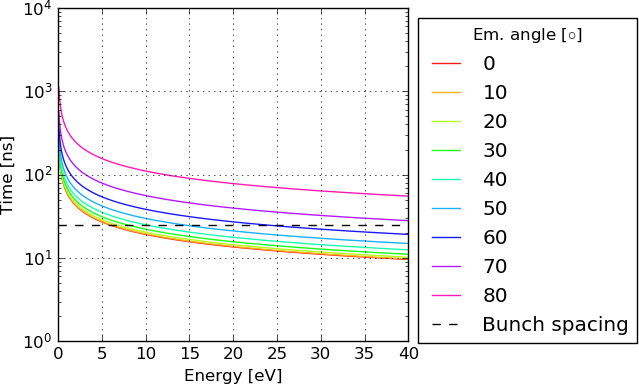
\includegraphics[width=0.55\textwidth]{../plots/time.png}
    \caption{The time needed for a photoelectron in a dipole e-cloud stripe to reach the opposing wall in dependence of the emission angle relative to the surface normal, in absence of electric fields.}
    \label{fig:time}
\end{figure}



\subsection{Distribution of photoelectrons in the chamber.}
\label{sec:photon_cdf}

Another idea would be to simulate the distribution of absorbed photons, and therefore the positions of new electron macroparticles.
So far, either a cosine squared or a uniform distribution of $\Psi$ in Fig.~\ref{fig:gt} has been used in most simulations.
Based on the high reflectivity of the non-sawtooth parts of the LHC chamber (at least for grazing incident angles), a uniform distribution might be the best approximation for the time being.

%For the log-normal distribution, the parameters $\sigma_l$ and $\mu_l$ have to be used in order to achieve the same sample variance and mean as for a normal distribution characterized by $\sigma_n$ and $\mu_n$.
%\begin{align}
%    \sigma_l &= \sqrt{\log\left(\frac{\sigma_n^2}{\mu_n^2}+1\right)}
%    \\
%    \mu_l &= \log\mu_n - \frac{\sigma_l^2}{2}
%\end{align}
%A branch called "photoemission" on GitHub adds a new input parameter \textbf{energy\_distribution}, the choices are in addition also a monoenergetic and a rectangular distribution.



\clearpage
\section{Best estimates for photoemission simulations}
    
It is explained how the best estimates for the PyECLOUD input parameters mentioned in Sec.~\ref{sec:input} are defined based on the previously mentioned papers.
Only some of them take photon induced scrubbing into account.
The notation used in the following pages, see also Eq.~(\ref{eq:not1}-\ref{eq:yy}):
\begin{center}
    \begin{tabular}{cc}
        $Y_i$ ($Y_i^*$) & Photoelectrons per impinging (absorbed) photon on first impact \\
        $Y_r$ ($Y_r^*$)& Photoelectrons per impinging (absorbed) photon after initial reflection \\
        $R_i$ & Reflection rate of photons on first impact point. \\
        $R_r$ & Reflection rate of photons that have been reflected once. \\
        $N_i$ & Photoelectrons emitted on first impact of photons. \\
        $N_r$ & Photoelectrons emitted elsewhere. \\
        $N_t$ & Total number of emitted photoelectrons.\\
        $n_\gamma$ & Number of photons emitted per proton and m in a bending magnet.
    \end{tabular}
\end{center}


\subsection{Retrieving k\_pe\_st and refl\_frac from published experiment results}

In case of uniform material properties in the beam pipe, k\_pe\_st is computed as follows:
\begin{align}
    \textbf{k\_pe\_st} = n_\gamma \frac{Y}{1-R} = n_\gamma Y^*
\end{align}
This is because all photons are eventually absorbed, either on direct impact or after an arbitrary number of reflections, and the material properties are uniform.
\begin{align}
    \textbf{refl\_frac} = \frac{N_r}{N_i+N_r} = \frac{R_iY^*_r}{(1-R_i)Y_i^* + R_iY^*_r}
\end{align}
However in the case of the sawtooth configuration in the LHC beam screen, the material properties are different at the  spot where the synchrotron radiation impacts first.
This means that number of photons absorbed at the impact point and after initial reflection have to be weighted with the photoelectron yields $Y^*$ and the reflectivity probability.
\begin{align}
    \textbf{k\_pe\_st} &= N_i + N_r
    \\
    &= N_\gamma \left( (1-R_i)Y_i^* + R_iY^*_r \right)
    \\
    &= N_\gamma \left( Y_i + R_iY^*_r \right)
    \label{eq:parts}
\end{align}
One simplification is that photons are not reflected back to the sawtooth material, given its relatively small portion relative to the total circumference.
This corresponds to $R_r=0$.
%Quantitatively, k\_pe\_st and refl\_frac are assessed in Sec.~\ref{sec:parameters}.

For \textbf{alimit}, the critical angle of the synchrotron radiation from Eq.~(\ref{eq:crit_angle}) could be used for $\omega = W_\text{Cu}/\hbar$: 0.36~mrad.
For \textbf{e\_pe\_sigma} and \textbf{e\_pe\_max}, describing the kinetic energy distribution of new electron macroparticles, 5 and 7~eV have been chosen in past simulations.
As stated before, the fact that photoelectrons are immediately being accelerated by the positively charged proton beam, means that their kinetic energy is of minor influence.

For the angular distribution of photoelectrons that are generated by reflected photons
\\
(\textbf{inv\_CDF\_ refl\_photoem\_file}), a uniform distribution should be used while a realistic distribution is not available.
This approach should be better than using the cosine distribution, since the probability of multiple reflections is much higher than single reflection upon impact, since the reflectivity was measured to be larger than 80\% for the non-sawtooth material.
A 2D cosine distribution should in any case be avoided, see Eq.~(\ref{eq:angles}).


\subsection{Consistency of different measurements}

The different published experimental results on photoelectron yields and reflectivities are compared in this table.
If two values are stated for a photoelectron yield, they correspond to the measurements before and after photon scrubbing.
The reflectivities colored in red only include the forward reflectivity.
The yields in blue were not published but could be retrieved with the simple relation between $R$, $Y$ and $Y^*$ from Eq.~(\ref{eq:yy}).
\begin{center}
    \begin{tabular}{c|ccc|ccc}
        \multirow{2}{*}{Source} & \multicolumn{3}{c|}{Cu co-lam.} & \multicolumn{3}{|c}{with sawtooth} \\
        & $R$ [\%] & $Y$ [e/ph]& $Y^*$ [e/ph]& $R$ [\%]& $Y$ [e/ph]& $Y^*$ [e/ph] \\\hline
        Baglin 1998 & {\color{red}80.9} & {\color{blue}0.022} & 0.114 & {\color{red}1.8} & {\color{blue} 0.052} & 0.053 \\
        Cimino 1999 & - & 0.103/0.063 & - & - & - & - \\
        Baglin 2001 & - & - & - & {\color{red}8} & {\color{blue}0.021/0.011} & 0.029/0.015 \\
        Mahne 2004 & 82 & - & - & 10 & - & - \\
    \end{tabular}
\end{center}

The differences between the Cimino and Baglin results can at least in parts be explained with different "as-received" samples of Cu, but of course also different measurement techniques may have been used.
Since only the two Baglin papers include results for sawtooth materials, these should be used for the simulation.
The reflectivities from the Mahne paper should be used because of the superior measurement apparatus for reflected photons.

\subsection{Parameters to use for the simulations}
\label{sec:parameters}
For a \textbf{conservative estimate}, the following table uses the high reflectivities from the Mahne paper and the high photoelectron yields $Y$ from the first Baglin paper, retrieved from the values for $Y^*$ as published in \cite{baglin}.
%The notation is the one used in Eq.~(\ref{eq:k}), with the subscripts $i$ and $r$ meaning "on impact" and "after reflection".

\begin{tabular}{c|cccc|cc}
Chamber type & $R_i$ & $R_r$ & $Y_i$ & $Y_r$ & $Y_i^*$ & $Y_r^*$  \\ \hline 
Cu co-lam. with sawtooth &10.0 &82.0 &5.2e-02 &2.2e-02& 5.8e-02 &1.2e-01 \\
Cu co-lam. &82.0 &82.0 &2.3e-02 &2.3e-02& 1.3e-01 &1.3e-01 \\
%	chamber & $R_i$ & $R_r$ & $Y_i$ & $Y_r$ & $Y_i^*$ & $Y_r^*$ & $N_i$ & $N_r$ & $N_t$ & $N_\gamma$ & relf\_frac & k\_pe\_st \\ \hline 
%	uniform &82.0 &82.0 &2.3e-02 &2.3e-02 &1.3e-01 &1.3e-01 &2.3e-02 &1.0e-01 &1.3e-01 &1.1e-02 &8.20e-01 &1.38e-03\\
%	with sawtooth &10.0 &82.0 &5.2e-02 &2.2e-02 &5.8e-02 &1.2e-01 &5.2e-02 &1.2e-02 &6.4e-02 &1.1e-02 &1.89e-01 &7.00e-04\\
\end{tabular}

These yields and reflectivities, together with the number of photons from Eq.~(\ref{eq:ngamma}), finally lead to the needed parameters refl\_frac and k\_pe\_st.

\begin{tabular}{c|ccc|c|cc}
Chamber type & $N_i$ & $N_r$ & $N_t$ & $n_\gamma$ & refl\_frac & k\_pe\_st \\ \hline 
Cu co-lam. with sawtooth& 5.2e-02 &1.2e-02 &6.4e-02 &1.1e-02 &1.89e-01 &7.00e-04\\
Cu co-lam.& 2.3e-02 &1.0e-01 &1.3e-01 &1.1e-02 &8.20e-01 &1.38e-03\\
\end{tabular}


A \textbf{realistic estimate} would include scrubbing effects and a much lower yield, as measured in the second Baglin paper.
With respect to the first, the yield of the sawtooth material is by a factor of $0.052/0.011 \approx 4.7$ lower.
If this factor is also applied to the yield of the other material, the following input parameters should be used.
In practise, mostly the value for $N_r$ is relevant as it denotes the amount of photoelectrons that contributes to the stripes in e-cloud simulations for dipoles and quadrupoles.

\begin{tabular}{c|cccc|cc}
Chamber type & $R_i$ & $R_r$ & $Y_i$ & $Y_r$ & $Y_i^*$ & $Y_r^*$  \\ \hline 
Cu co-lam. with sawtooth& 10.0 &82.0 &1.0e-02 &4.6e-03& 1.1e-02 &2.6e-02 \\
Cu co-lam.& 82.0 &82.0 &4.6e-03 &4.6e-03& 2.6e-02 &2.6e-02 \\
%	chamber & $R_i$ & $R_r$ & $Y_i$ & $Y_r$ & $Y_i^*$ & $Y_r^*$ & $N_i$ & $N_r$ & $N_t$ & $N_\gamma$ & relf\_frac & k\_pe\_st \\ \hline 
%	with sawtooth &10.0 &82.0 &1.0e-02 &6.2e-03 &1.1e-02 &3.5e-02 &1.0e-02 &3.5e-03 &1.4e-02 &1.1e-02 &2.55e-01 &1.48e-04\\
\end{tabular}

\begin{tabular}{c|ccc|c|cc}
Chamber type & $N_i$ & $N_r$ & $N_t$ & $n_\gamma$ & refl\_frac & k\_pe\_st \\ \hline 
Cu co-lam. with sawtooth& 1.0e-02 &2.6e-03 &1.3e-02 &1.1e-02 &2.03e-01 &1.39e-04\\
Cu co-lam.& 4.6e-03 &2.1e-02 &2.6e-02 &1.1e-02 &8.20e-01 &2.81e-04\\
\end{tabular}

However it should be noted that this alteration is speculative, and should be confirmed with measurements.




%\subsection{Excluding scrubbing effects}
%
%The results from Sec.~\ref{sec:Baglin}, as shown in Sec.~\ref{sec:Mahne}, underestimate the reflectivities.
%According to Eq.~(\ref{eq:yy}), this also results in too low values for $Y^*$.
%Therefore, the yields have been corrected:
%\begin{align}
%	Y^*_\text{new} = Y^*_\text{old} \frac{1-R_\text{old}}{1-R_\text{new}}
%    \label{eq:}
%\end{align}
%
%The resulting vaues for refl\_frac and k\_pe\_st are stated in Tab.~\ref{tab:input_table}, together with intermediate results.
%"Cu co-lam. with sawtooth" corresponds to an LHC chamber with sawtooth structure only at the impact point of the photoelectrons, as it is the case for the majority of the installed material.
%
%\begin{table}[tbh]
%    \centering
%        \tiny
%    \begin{tabular}{ccccccccccccc}
%	%Type & $R_i$ & $R_r$ & $Y_i$ & $Y_r$ & $Y_i^*$ & $Y_r^*$ & $N_i$ & $N_r$ & $N_t$ & $N_\gamma$ & $R$ & k\_pe\_st \\ \hline 
%    Type & {\color{blue}$R_i$} & {\color{blue}$R_r$} & {\color{red}$Y_i$} & {\color{red}$Y_r$} & $Y_i^*$ & $Y_r^*$ & $N_i$ & $N_r$ & $N_t$ & $N_\gamma$ & refl\_frac & k\_pe\_st \\ \hline 
%	Cu co-lam. with sawtooth &10.0 &82.0 &5.2e-02 &2.2e-02 &5.8e-02 &1.2e-01 &5.2e-02 &1.2e-02 &6.4e-02 &1.1e-02 &1.9e-01 &7.0e-04\\
%	Cu co-lam. &82.0 &82.0 &2.3e-02 &2.3e-02 &1.3e-01 &1.3e-01 &2.3e-02 &1.0e-01 &1.3e-01 &1.1e-02 &8.2e-01 &1.4e-03\\
%    \end{tabular}
%    \caption{
%        These parameters correspond to the measurements from Baglin et al (red), while accounting for the underestimated photon reflectivity (blue).
%        The notation is also used in Eq.~(\ref{eq:k}).
%        $N_i$ and $N_r$ are the photoelectrons per photon on impact and after reflection.
%        $N_\gamma$ is the number of photoelectrons per proton and meter, see Eq.~(\ref{eq:ngamma}).
%    }
%    \label{tab:input_table}
%\end{table}
%
%\subsection{Including scrubbing effects}
%If scrubbing effects are taken into account, the photoemission yield should be lower by roughly 40\%, as supported by the papers presented in Sec.~\ref{sec:Baglin2} and \ref{sec:Cimino}.


\clearpage
\addcontentsline{toc}{section}{References}
\bibliographystyle{elsarticle-num}
\bibliography{lit}

\end{document}

